% !TeX spellcheck = it_IT
\newpage
\section{FaaS}
L'approccio FaaS è un mercato in crescita e ad oggi esistono molteplici opzioni tra le quali scegliere. In particolare le suddividiamo in due categorie: \emph{commerciali} (e.g. AWS Lambda) e \emph{open source} (e.g. Apache Openwisk).\\
Per fare una scelta consapevole, dobbiamo analizzare le proposte da due punti di vista: quello commerciale e quello tecnico.
\subsection{Business view}
\subsubsection{Licensing}
Tutte le piattaforme \textbf{open source} usano licenze abbastanza permissive, come ad esempio Apache 2.0. Quelle \textbf{commerciali} invece usano software proprietario, fatta eccezione per MS Azure Functions che ha alcune componenti libere.
\begin{center}
	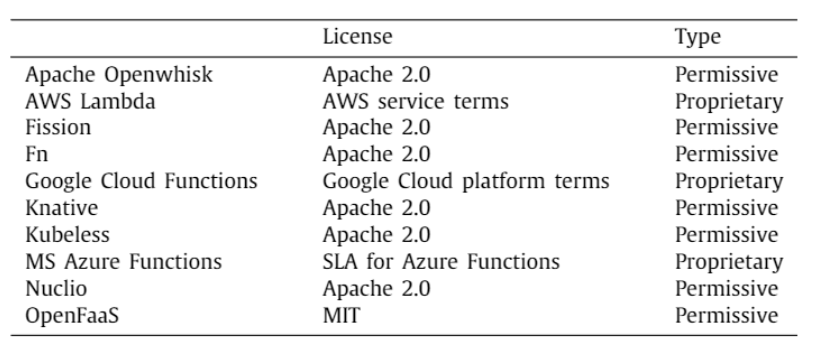
\includegraphics[scale=0.4]{faas_licensing.png}
\end{center}
\subsubsection{Installazione}
Tra le opzioni commerciali solamente Azure functions ha dei servizi installabili \emph{on-premises}. Quelle open source supportano invece molteplici host, con Kubernetes tra i più popolari.
\begin{center}
	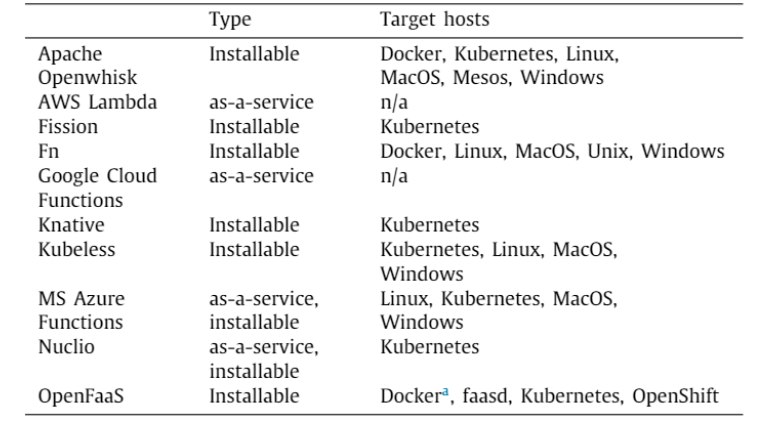
\includegraphics[scale=0.4]{faas_installation.png}
\end{center}
\newpage
\subsubsection{Source code}
Tutte le piattaforme open source sono hostate su GitHub ed implementate in Go.
\begin{center}
	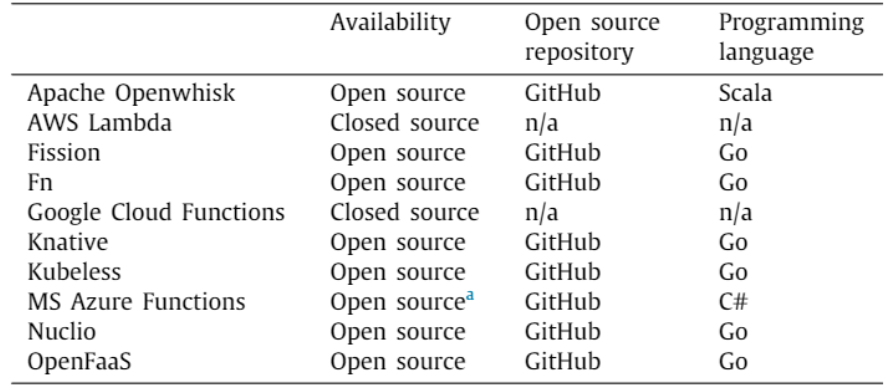
\includegraphics[scale=0.4]{faas_opensource.png}
\end{center}
\subsubsection{Interfaccia}
Tutte le piattaforme forniscono CLI, mentre API e GUI  non sono sempre presenti in quelle open source. Inoltre in queste ultime il metodo di amministrazione cambia molto tra l'una e l'altra.
\begin{center}
	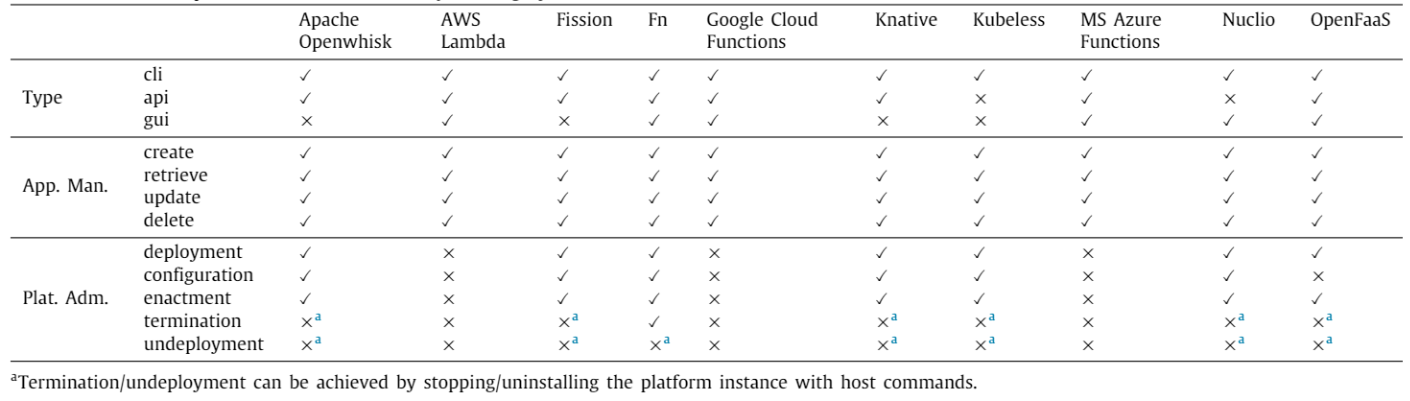
\includegraphics[scale=0.3]{faas_interface.png}
\end{center}
\subsubsection{Community}
Le piattaforme open source sono molto ben votate su GitHub ma poco cercate e diffuse su StackOverflow, a differenza di quelle commerciali.
\begin{center}
	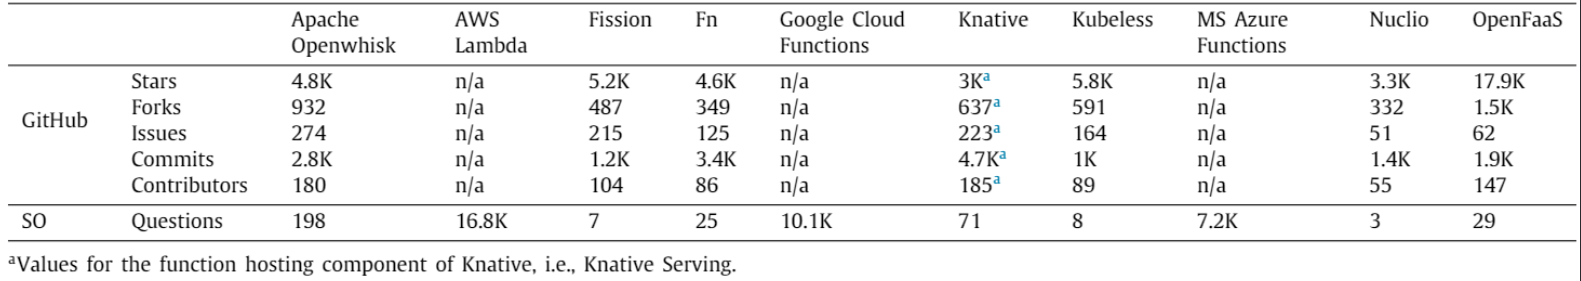
\includegraphics[scale=0.3]{faas_community.png}
\end{center}
\subsubsection{Documentazione}
Tutte le piattaforme forniscono la documentazione per l'utilizzo e il deploy del servizio ma non tutte le loro architetture sono documentate.
\begin{center}
	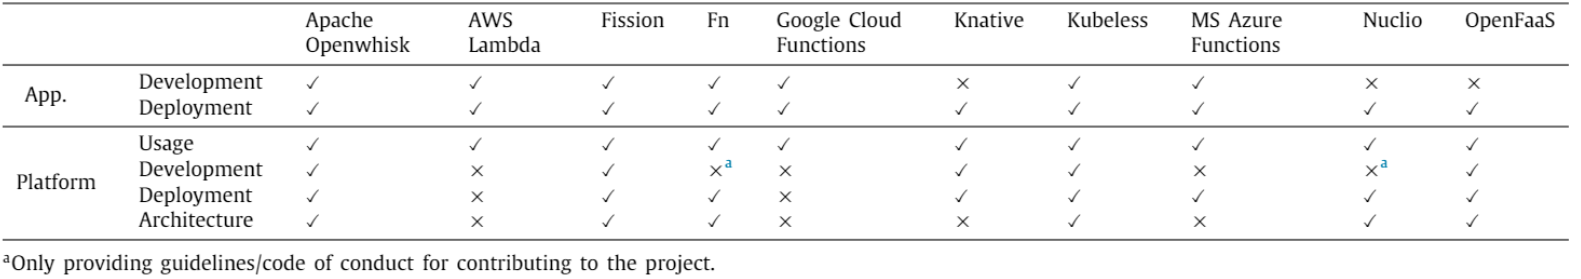
\includegraphics[scale=0.25]{faas_documentation.png}
\end{center}
\subsection{Technical view}
\subsubsection{Sviluppo}
I linguaggi più comuni nello sviluppo in ambito FaaS sono Java, NodeJS e Python, con il supporto di Docker.
\begin{center}
	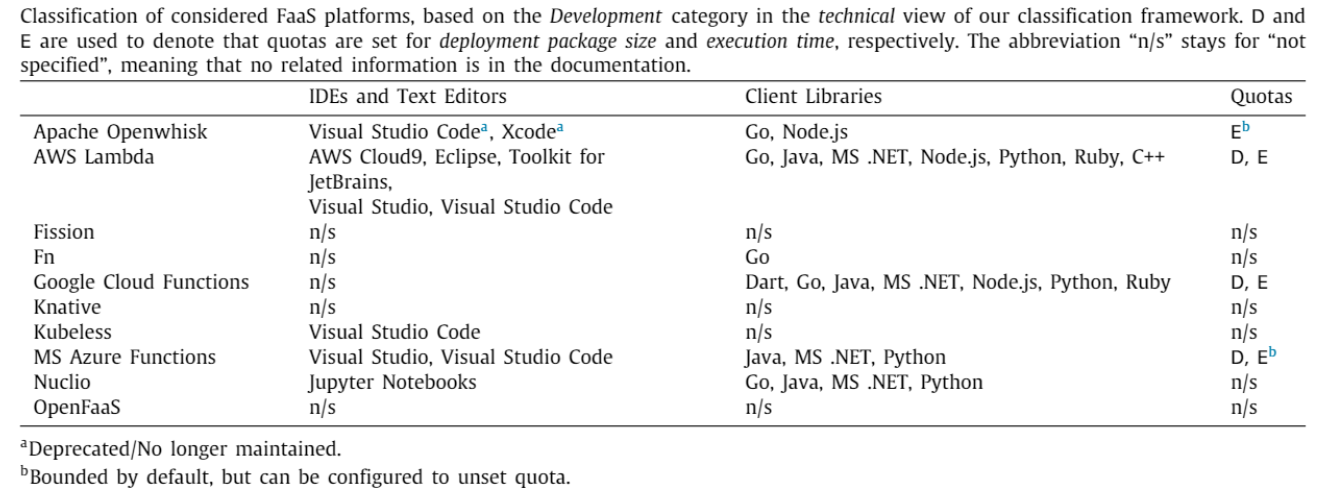
\includegraphics[scale=0.33]{faas_developement.png}
\end{center}
\subsubsection{Versioning}
La maggior parte delle piattaforme implementano un sistema di versioning in maniera implicita, al contrario di quelle commerciali:
\begin{itemize}
	\item \textbf{Dedicated mechanisms}
	\item \textbf{Implicit mechanisms}
\end{itemize}
\begin{center}
	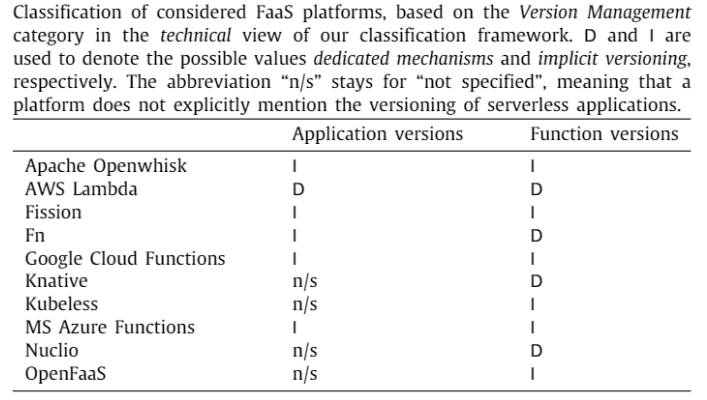
\includegraphics[scale=0.4]{faas_versioning.png}
\end{center}
\subsubsection{Event sources}
Tutte le piattaforme supportano la chiamata di funzioni tramite richieste \textbf{sincrone} HTTP, mentre solo alcune supportano quelle \textbf{asincrone}. Più della metà non supportano il salvataggio dei \textbf{dati delle richieste}. Gli \textbf{scheduler}, gli \textbf{stream processing} e il \textbf{messaging} sono ampiamente supportati. Più della metà delle piattaforme documentano la possibilità di creare \textbf{eventi personalizzati}.
\newpage
\subsubsection{Function orchestration}
Più della metà delle piattaforme supportano il function orchestration tramite DSL proprietari o funzioni apposite.
\begin{center}
	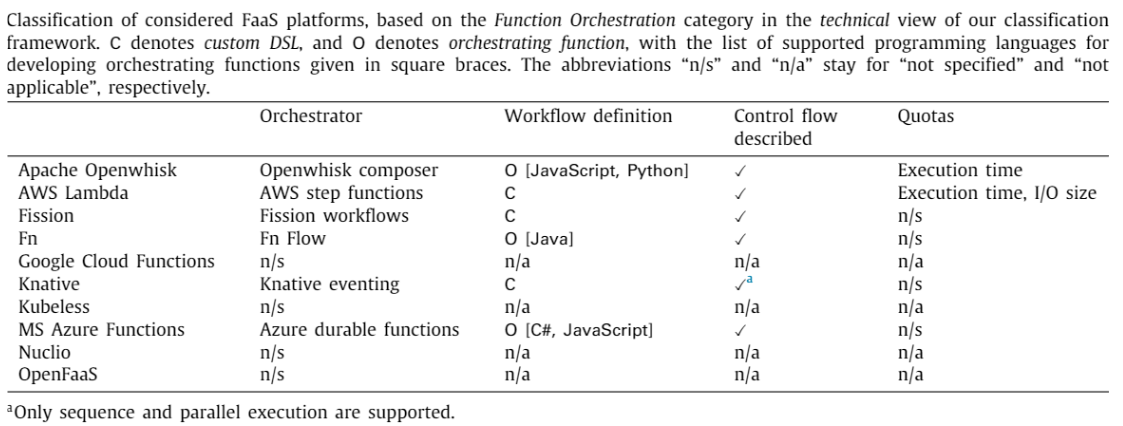
\includegraphics[scale=0.38]{faas_orchestration.png}
\end{center}

\subsubsection{Testing e debugging}
La maggior pare delle piattaforme supporta testing funzionale e debugging delle funzioni. La differenza sta nella sofisticatezza di questi sistemi, che è più elevata per le piattaforme commerciali.
\subsubsection{Logging}
Le piattaforme commerciali usano strumenti ad hoc per monitorare lo stato del servizio mentre quelle open source si rifanno a servizi terzi.
\begin{center}
	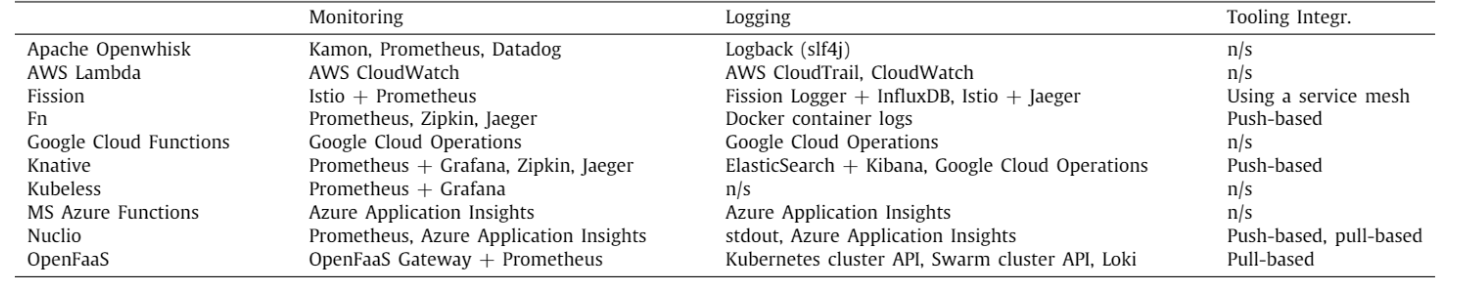
\includegraphics[scale=0.3]{faas_logging.png}
\end{center}
\subsubsection{Application delivery}
La maggior parte delle piattaforme segue un approccio dichiarativo per automatizzare il deploy delle applicazioni. Solo quelle commerciali supportano la pipeline di tipo CI/CD (Continuous Implementation/Continuous Deployment).
\begin{center}
	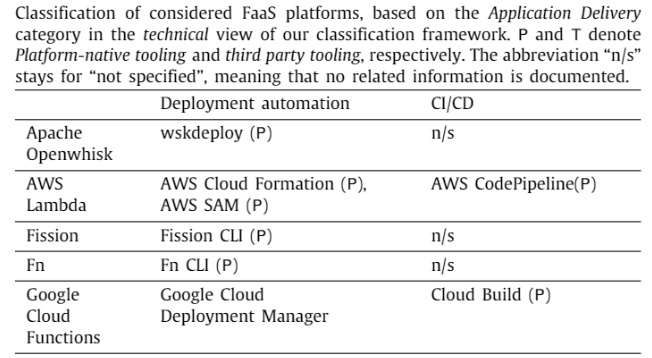
\includegraphics[scale=0.3]{faas_deployment_1.png}
	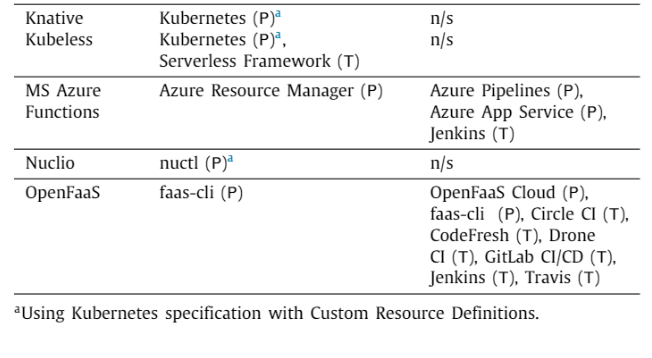
\includegraphics[scale=0.3]{faas_deployment_2.png}
\end{center}
\subsubsection{Riuso}
Solamente AWS Lambda e MS Azure Functions prevedono un marketplace per condividere e riutilizzare funzioni.
\subsubsection{Gestione degli accessi}
Le piattaforme commerciali supportano nativamente l'autenticazione e il controllo delle risorse. Quelle open source di solito sfruttano features del sistema operativo.
